\PassOptionsToPackage{unicode=true}{hyperref} % options for packages loaded elsewhere
\PassOptionsToPackage{hyphens}{url}
%
\documentclass[ignorenonframetext,aspectratio=169]{beamer}
\usepackage{pgfpages}
\setbeamertemplate{caption}[numbered]
\setbeamertemplate{caption label separator}{: }
\setbeamercolor{caption name}{fg=normal text.fg}
\beamertemplatenavigationsymbolsempty
% Prevent slide breaks in the middle of a paragraph:
\widowpenalties 1 10000
\raggedbottom
\setbeamertemplate{part page}{
\centering
\begin{beamercolorbox}[sep=16pt,center]{part title}
  \usebeamerfont{part title}\insertpart\par
\end{beamercolorbox}
}
\setbeamertemplate{section page}{
\centering
\begin{beamercolorbox}[sep=12pt,center]{part title}
  \usebeamerfont{section title}\insertsection\par
\end{beamercolorbox}
}
\setbeamertemplate{subsection page}{
\centering
\begin{beamercolorbox}[sep=8pt,center]{part title}
  \usebeamerfont{subsection title}\insertsubsection\par
\end{beamercolorbox}
}
\AtBeginPart{
  \frame{\partpage}
}
\AtBeginSection{
  \ifbibliography
  \else
    \frame{\sectionpage}
  \fi
}
\AtBeginSubsection{
  \frame{\subsectionpage}
}
\usepackage{lmodern}
\usepackage{amssymb,amsmath}
\usepackage{ifxetex,ifluatex}
\usepackage{fixltx2e} % provides \textsubscript
\ifnum 0\ifxetex 1\fi\ifluatex 1\fi=0 % if pdftex
  \usepackage[T1]{fontenc}
  \usepackage[utf8]{inputenc}
  \usepackage{textcomp} % provides euro and other symbols
\else % if luatex or xelatex
  \usepackage{unicode-math}
  \defaultfontfeatures{Ligatures=TeX,Scale=MatchLowercase}
\fi
\usetheme[]{Frankfurt}
\usecolortheme{beaver}
% use upquote if available, for straight quotes in verbatim environments
\IfFileExists{upquote.sty}{\usepackage{upquote}}{}
% use microtype if available
\IfFileExists{microtype.sty}{%
\usepackage[]{microtype}
\UseMicrotypeSet[protrusion]{basicmath} % disable protrusion for tt fonts
}{}
\IfFileExists{parskip.sty}{%
\usepackage{parskip}
}{% else
\setlength{\parindent}{0pt}
\setlength{\parskip}{6pt plus 2pt minus 1pt}
}
\usepackage{hyperref}
\hypersetup{
            pdftitle={Biotechnology types},
            pdfauthor={Deependra Dhakal},
            pdfborder={0 0 0},
            breaklinks=true}
\urlstyle{same}  % don't use monospace font for urls
\newif\ifbibliography
\setlength{\emergencystretch}{3em}  % prevent overfull lines
\providecommand{\tightlist}{%
  \setlength{\itemsep}{0pt}\setlength{\parskip}{0pt}}
\setcounter{secnumdepth}{0}

% set default figure placement to htbp
\makeatletter
\def\fps@figure{htbp}
\makeatother

% % set background image if you will
% \usebackgroundtemplate%
% {%
%     \includegraphics[width=\paperwidth,height=\paperheight]{02-dna_modification_background_dna_helix.jpg}%
% }

% % set caption font size
% % note that beamer presentation native captions have their own configs
% \usepackage{caption}
% \captionsetup{font=footnotesize}

% this font option is amenable for beamer
\setbeamerfont{caption}{size=\tiny}

% some beamer themes naturally might not support navigation symbols
% \setbeamertemplate{navigation symbols}{} % remove navigation symbols

\setbeamertemplate{footline}[page number] % insert page number in footline

% \setbeamertemplate{navigation symbols}{slide} % insert slide indication in navigation
% \setbeamertemplate{navigation symbols}{frame} % insert frame indication in navigation
% \setbeamertemplate{navigation symbols}{section} % insert section indication in navigation
% \setbeamertemplate{navigation symbols}{subsection} % insert subsection indication in navigation

% \AtBeginSubsection{} % supress subsection display

\title{Biotechnology types}
\author{Deependra Dhakal}
\providecommand{\institute}[1]{}
\institute{GAASC, Baitadi \and Tribhuwan University}
\date{Academic year 2019-2020}

\begin{document}
\frame{\titlepage}

\begin{frame}
\tableofcontents[hideallsubsections]
\end{frame}
\hypertarget{environmental-biotechnology}{%
\section{Environmental
biotechnology}\label{environmental-biotechnology}}

\hypertarget{overview}{%
\subsection{Overview}\label{overview}}

\begin{frame}{Background}
\protect\hypertarget{background}{}

\begin{itemize}
\tightlist
\item
  People have always been fascinated by the environment around them and
  successful in harnessing the environment for our benefit.
\item
  Curiosity to explore uncharted life forms drives our motivations.
\item
  Virosphere! How big is it?
\item
  Human body harbors \(10^14\) bacteria, while our own only comprise
  \(10^13\).
\end{itemize}

\end{frame}

\hypertarget{applications}{%
\subsection{Applications}\label{applications}}

\begin{frame}{Wide applications}
\protect\hypertarget{wide-applications}{}

\begin{itemize}
\tightlist
\item
  An increase in the productivity of crops, without an increase in the
  dependency on environmentally-damaging agrochemicals.
\item
  As a result of increased productivity, a reduced pressure to exploit
  the remaining uncultivated habitats.
\item
  As a result of increased productivity, a reduction in energy inputs
  (mostly from reduced agrochemical manufacture).
\item
  The creation of alternative, renewable, sources of energy (e.g.,
  biodiesel).
\item
  The creation of new more environment-friendly raw materials for
  industry (e.g., biodegradable plastics from plant starches, or
  high-value speciality chemicals).
\item
  As a result of the development of genetically-modified crops (if
  properly used), a reduction in the amount of agrochemical (e.g.,
  pesticides and herbicides) released into the environment.
\end{itemize}

\end{frame}

\begin{frame}{Bio-environmental processes}
\protect\hypertarget{bio-environmental-processes}{}

\alert{Bioremediation}

\begin{itemize}
\tightlist
\item
  One of the avenues in biotechnology that has made rapid advances
\item
  ``biological'' means of cleaning the environment.
\item
  Naturally occurring microorganisms often have the ability to degrade
  human-made pollutants.
\item
  \emph{Rhodococcus} sp. has a highly diverse pathways to degrade
  pollutants, such as short- and long-chain alkanes, aromatic molecules
  (both halogenated and nitro-substituted), and heterocyclic and
  polycyclic aromatic compounds, including quino lone, pyridine,
  thiocarbamate, s-triazine herbicides, 2-mercaptobenzothiazole (a
  rubber vulcanization accelerator), benzothiophene, dibenzothiophene,
  MTBE, and the related ethyl tert-butyl ether (ETBE).
\end{itemize}

\end{frame}

\begin{frame}{Bio-environmental processes}
\protect\hypertarget{bio-environmental-processes-1}{}

\begin{itemize}
\tightlist
\item
  \alert{Biostimulation} is the release of nutrients, oxidants, or
  electron donors into the environment to stimulate naturally occurring
  microorganisms to degrade a contaminant.
\item
  \alert{Bioaugmentation} is adding specific microorganisms plus their
  energy sources to decontaminate a polluted area.
\item
  \alert{Microbial fuel cells} create electricity through the use of
  microorganisms. Organisms that transfer electrons to the anode are
  called electrode-reducing organisms. They can pass electrons through a
  mediator molecule in the solution, directly through proteins in their
  outer membrane, or through nanowires or pili that coat the outer
  surface of the bacterium. Electrode-oxidizing organisms take electrons
  from the cathode to reduce various substances, such as carbon dioxide
  to acetate.
\end{itemize}

\end{frame}

\begin{frame}{Biofuel production}
\protect\hypertarget{biofuel-production}{}

\begin{figure}
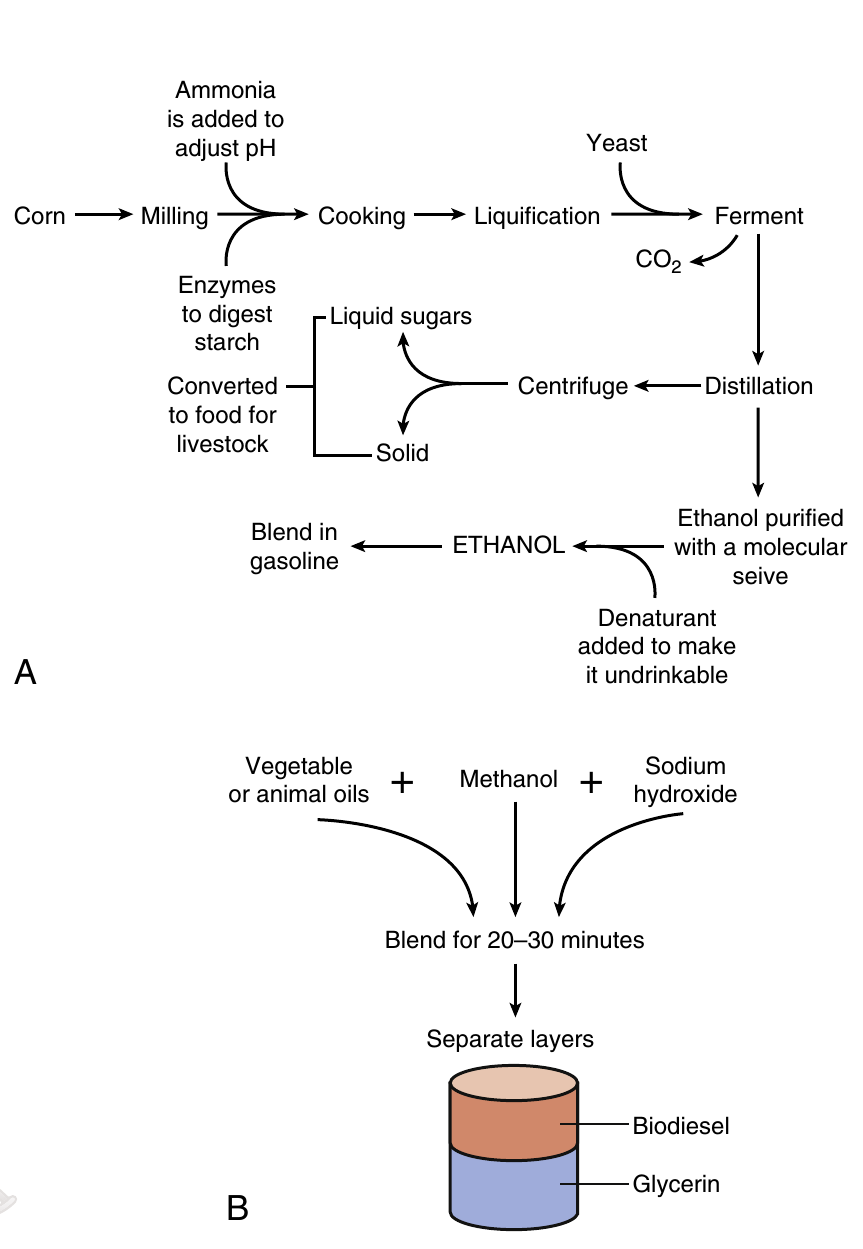
\includegraphics[width=0.28\linewidth]{../images/biofuel_production} \caption{\textbf{(A)} Production of ethanol from corn requires the addition of ammonia to adjust the pH and enzymes to help digest starch and yeast to ferment the corn mash. \textbf{(B)} Biodiesel is created by the blending of methanol, sodium hydroxide, and vegetable oil for 20-30 minutes.}\label{fig:biofuel-production}
\end{figure}

\end{frame}

\begin{frame}{Mechanism}
\protect\hypertarget{mechanism}{}

\begin{itemize}
\tightlist
\item
  PCR is routinely used to amplify random sequences from many
  environmental samples in the hope of identifying new genes.
\item
  After PCR DNA is sequenced.
\item
  Then bioinformatics reveals whether or not the sequence (or a close
  relative) has already been identified or if it is completely novel.
\item
  Microarrays are used to compare numbers and types of organisms present
  in different environment.
\end{itemize}

\end{frame}

\begin{frame}{Identifying new genes with metagenomics}
\protect\hypertarget{identifying-new-genes-with-metagenomics}{}

\begin{itemize}
\tightlist
\item
  Allows identification of microorganisms, viruses, or free DNA that
  exist in the natural environment.
\item
  Approaches: next-generation DNA sequencing, PCR, RT-PCR and
  microarrays
\item
  Metagenomics is the process of statistically combining separate
  genomic analyses; deals with a mixture of DNA forms.
\item
  Study of marine microbiology, human gut microbiology, assessment of
  how microorganisms form symbiotic relationships with their hosts,
  finding novel antibiotics or enzymes, replacement of chemical
  pesticides with crops genetically engineered for tolerance to
  microorganisms and nematodes, etc.
\end{itemize}

\end{frame}

\begin{frame}{Current concerns and Solutions}
\protect\hypertarget{current-concerns-and-solutions}{}

\begin{columns}[T,onlytextwidth]
  \column{0.5\textwidth}
  
  \alert {Concerns}
  \begin{itemize}
  \item Herbicide use
  \item Genetic pollution and superweeds
  \item Antibiotic resistance
  \item Unexpected effects
  \item Pest resistance
  \item Persistence and weediness
  \item Damage to wildlife and biodiversity
  \end{itemize}
  
  \column{0.5\textwidth}
  
  \alert {Avenues}
  \begin{itemize}
  \item Genetic modification of plants achieves essentially the same result as conventional plant breeding
  \item Wide-crossing
  \item In Nature, genes are exchanged between species
  \item Gene instability in conventional crops
  \item Conventional breeding is not 'Natural' either
  \item Gene transfer from crops to their 'Wild' relatives
  \item Novel, sustainable, agricultural practices needed
  
  \end{itemize}
  
\end{columns}

\end{frame}

\begin{frame}{Study techniques}
\protect\hypertarget{study-techniques}{}

\begin{figure}
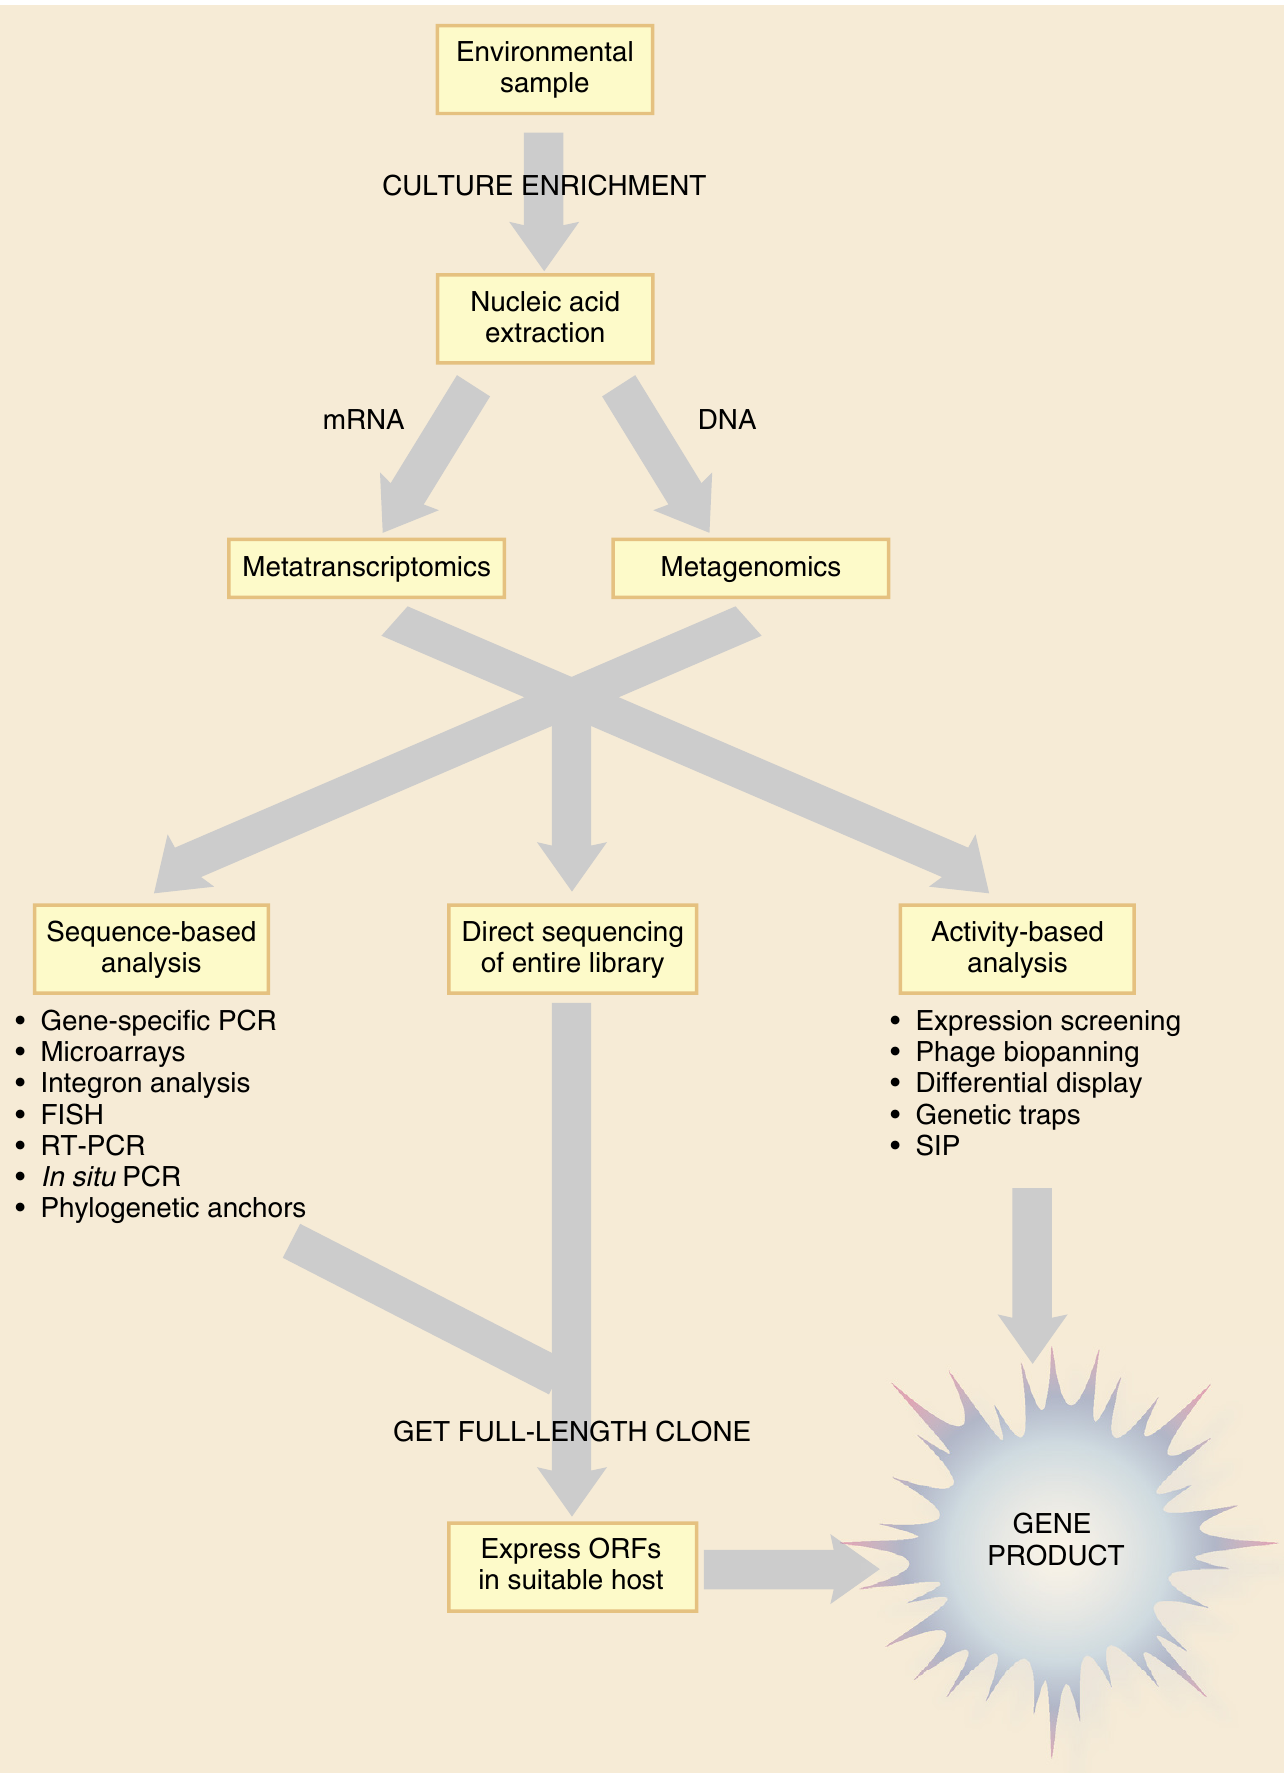
\includegraphics[width=0.32\linewidth]{../images/environmental_techniques} \caption{Techniques to study environmental samples}\label{fig:environment-samples-study}
\end{figure}

\end{frame}

\hypertarget{medical-biotechnology}{%
\section{Medical biotechnology}\label{medical-biotechnology}}

\hypertarget{applications-1}{%
\subsection{Applications}\label{applications-1}}

\begin{frame}{Popular technologies}
\protect\hypertarget{popular-technologies}{}

\begin{itemize}
\tightlist
\item
  Cheaper medicines from biotechnology
\item
  Medicines from `cultured' cells
\item
  Genetic modification for medicine production
\item
  Immune technology; Killed pathogens, attenuated pathogens, single
  proteins, or epitopes from a disease-causing pathogen are used as
  vaccines. They are isolated and injected into people to elicit their
  immune response without causing the disease. Multivalent vaccines
  contain antigens to different proteins from a pathogen or family of
  pathogens.
\item
  Cancer technology; Oncogene detection, oncogene attenuation
\end{itemize}

\end{frame}

\begin{frame}{Popular technologies}
\protect\hypertarget{popular-technologies-1}{}

\begin{itemize}
\tightlist
\item
  Gene therapy; Engineered retroviruses are the most frequently used
  viral vectors in gene therapy. Defective retrovirus vectors are grown
  in cells with an integrated helper virus to allow formation of virus
  particles.
\item
  ELISA assay; Antibodies are used in ELISA assays to determine the
  relative concentration of the target protein or antigen in a sample.
  Primary antibodies recognize the target protein or antigen. Secondary
  antibodies recognize the primary antibody and often carry a detection
  system. Secondary antibodies are made to recognize any antibody that
  is made in sheep, cow, rabbit, goat, or mouse.
\end{itemize}

\end{frame}

\begin{frame}{Stem cell therapy}
\protect\hypertarget{stem-cell-therapy}{}

\begin{itemize}
\tightlist
\item
  Characteristics of stem cells:

  \begin{itemize}
  \tightlist
  \item
    they maintain the ability to divide continually,
  \item
    they are undifferentiated, and
  \item
    they have the ability to differentiate into multiple cell types
  \end{itemize}
\item
  Embryonic stem cells are totipotent.
\item
  Adult or somatic stem cells are able to differentiate into different
  cell types but are multipotent; that is, they are restricted to the
  tissues in which they originate.
\item
  Embryonic stem cell lines are created from the inner cell mass of the
  blastula stage of an embryo from many different mammals, including
  humans, mice, and primates.
\item
  The cell lines can be induced to differentiate by forming embryoid
  bodies that ultimately differentiate into different cell types.
\end{itemize}

\end{frame}

\begin{frame}{Stem cell therapy}
\protect\hypertarget{stem-cell-therapy-1}{}

\begin{figure}
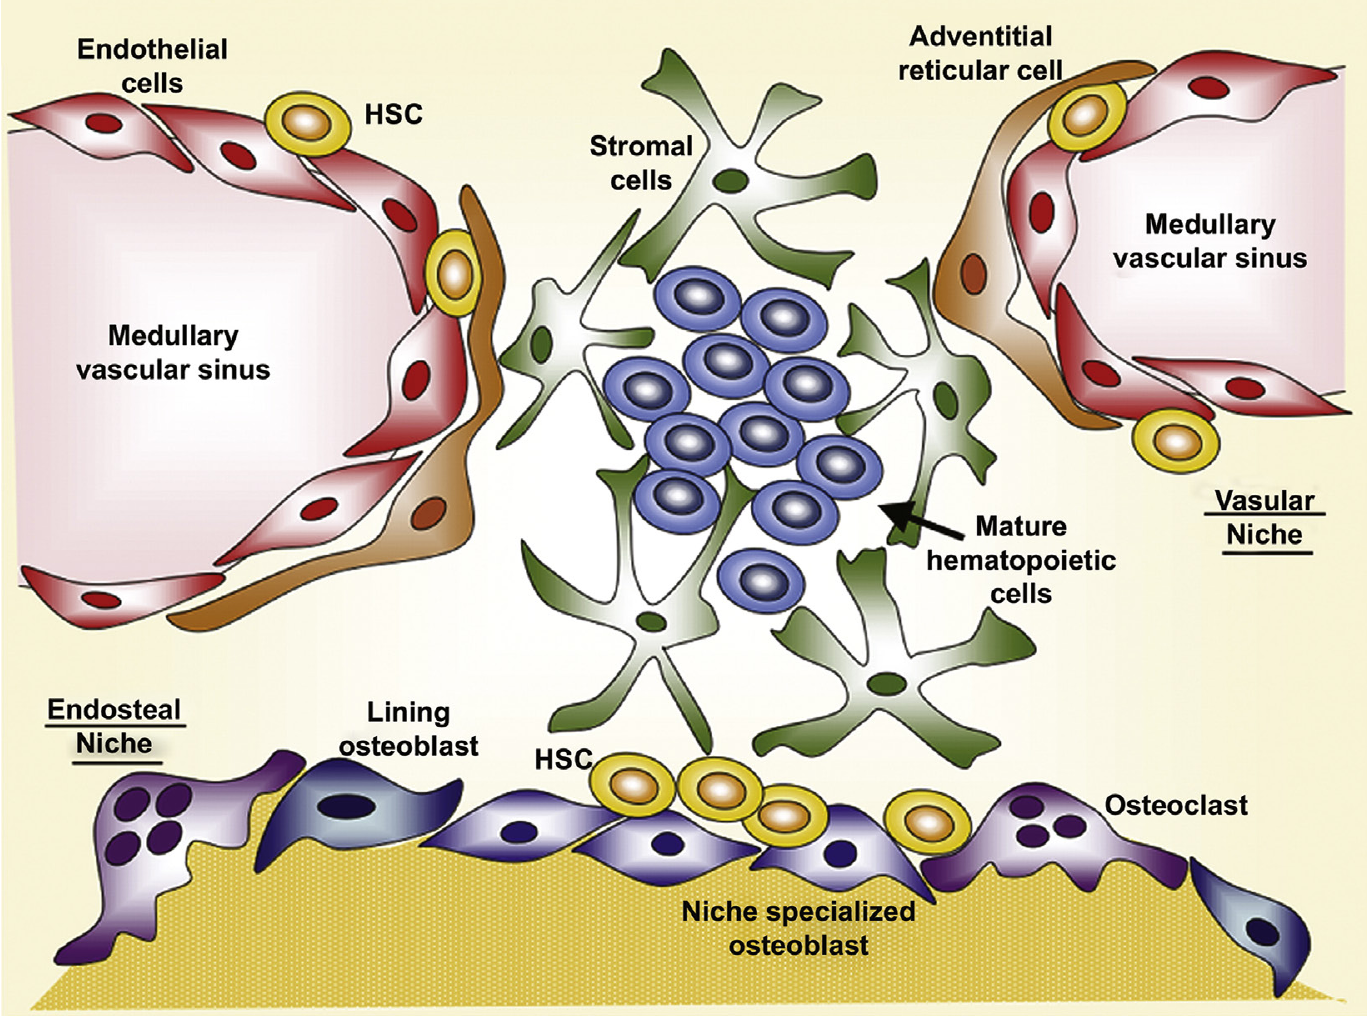
\includegraphics[width=0.45\linewidth]{../images/hematopoietic_stem_cells} \caption{\textbf{Hematopoietic stem cells} are located near the interface of the bone marrow and bone surface (the endosteal niche) and also near vascular sinuses (vascular niche). The HSCs in each niche divide to form mature hematopoietic cells that populate the marrow tissues.}\label{fig:stem-cell-therapy}
\end{figure}

\end{frame}

\begin{frame}{Cloning dolly}
\protect\hypertarget{cloning-dolly}{}

\begin{figure}
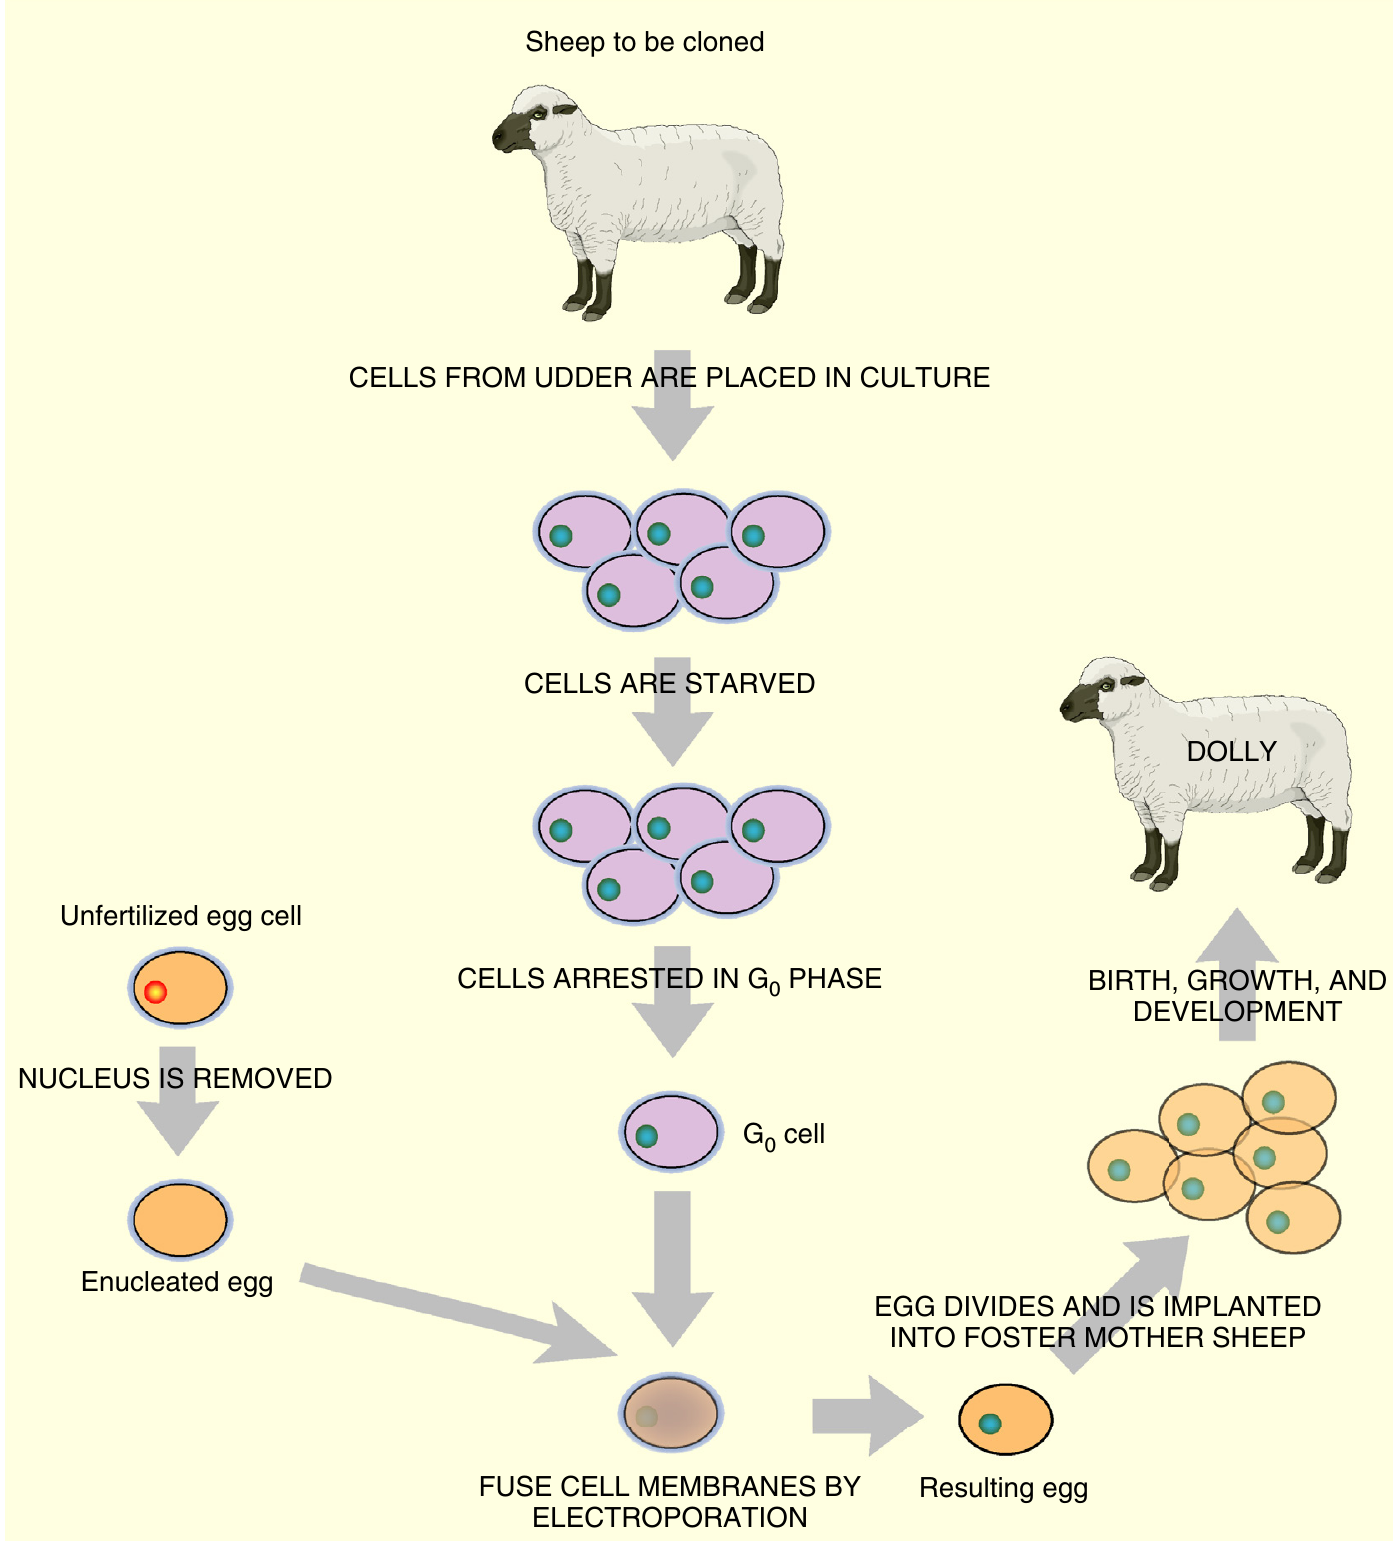
\includegraphics[width=0.38\linewidth]{../images/dolly_cloning} \caption{To clone a mammal such as a sheep, cells from the udder are isolated, grown in culture, and then starved in order to arrest them in $G_0$ of the cell cycle. Unfertilized egg cells from another sheep are also harvested, and the nucleus is removed. An electrical stimulus fuses the $G_0$ udder cell with the enucleated egg, thus placing a somatic cell nucleus into an undifferentiated cytoplasm. The eggs that result are put back into a foster mother, and the offspring are screened for DNA identical to the donor sheep.}\label{fig:dolly-sheep-cloning}
\end{figure}

\end{frame}

\hypertarget{forensic-biotechnology}{%
\section{Forensic biotechnology}\label{forensic-biotechnology}}

\begin{itemize}
\tightlist
\item
  Researches and uses the basis of identity to resolve conflicting
  situations and help create unique database of individuals.
\item
  Fingerprint patterns are multigenic trait.
\item
  Retinal scans take advantage of the unique pattern of blood vessels on
  the retina at the back of the eyes.
\item
  Blood typing provides identity based on presence of blood antigens
  groups.
\end{itemize}

\hypertarget{applications-2}{%
\subsection{Applications}\label{applications-2}}

\begin{frame}{DNA fingerprinting}
\protect\hypertarget{dna-fingerprinting}{}

\begin{itemize}
\tightlist
\item
  DNA fingerprinting relies on the unique pattern made by a series of
  DNA fragments after separating them according to length by gel
  electrophoresis.
\item
  The samples are then processed to generate a set of DNA fragments.
  When Alec Jeffreys invented DNA fingerprinting in 1985 in England, the
  DNA was cut with restriction enzymes to generate fragments because PCR
  had not yet been invented.
\item
  Nowadays, DNA is prepared by PCR, and fluorescent dyes are used for
  labeling. In addition, modern DNA fingerprinting uses repeated
  sequences (short tandem repeats or STRs) for routine identification
  purposes.
\end{itemize}

\end{frame}

\begin{frame}{DNA fingerprinting}
\protect\hypertarget{dna-fingerprinting-1}{}

\begin{itemize}
\tightlist
\item
  For the first generation of DNA fingerprints, restriction enzymes were
  used to generate the variation in DNA fragment size between
  individuals. Variations in the DNA base sequence of restriction enzyme
  recognition sites result in differences in the size of the fragments.
\item
  Such sequence differences are called restriction fragment length
  polymorphisms (\textbf{RFLPs}).
\item
  Many different restriction enzymes with distinct recognition sites are
  used on each DNA sample.
\item
  Even if mutations have changed a few bases of the target sequence
  around the cut site, there is usually still enough similarity for
  probes to bind.
\end{itemize}

\end{frame}

\begin{frame}{RFLP steps}
\protect\hypertarget{rflp-steps}{}

\begin{itemize}
\tightlist
\item
  The DNA is cut with a restriction enzyme.
\item
  The DNA fragments are separated by length or molecular weight by gel
  electrophoresis.
\item
  The fragments are visualized by Southern blotting. The separated
  fragments are transferred from the gel to nylon paper. Then a
  radioactively labeled DNA probe is added.
\item
  The probe binds to those DNA fragments with complementary sequences.
\item
  The blot is covered with radiation-sensitive film to give an
  autoradiograph. This shows the location of those DNA fragments that
  reacted with the radioactive probe.
\item
  The final product of a DNA fingerprint is an autoradiograph that
  contains at least five essential lanes (Figure
  \ref{fig:fingerprint-lanes}). The markers are standardized DNA
  fragments of known size, which have been radioactively labeled.
\end{itemize}

\end{frame}

\begin{frame}{RFLP fingerprinting}
\protect\hypertarget{rflp-fingerprinting}{}

\begin{figure}
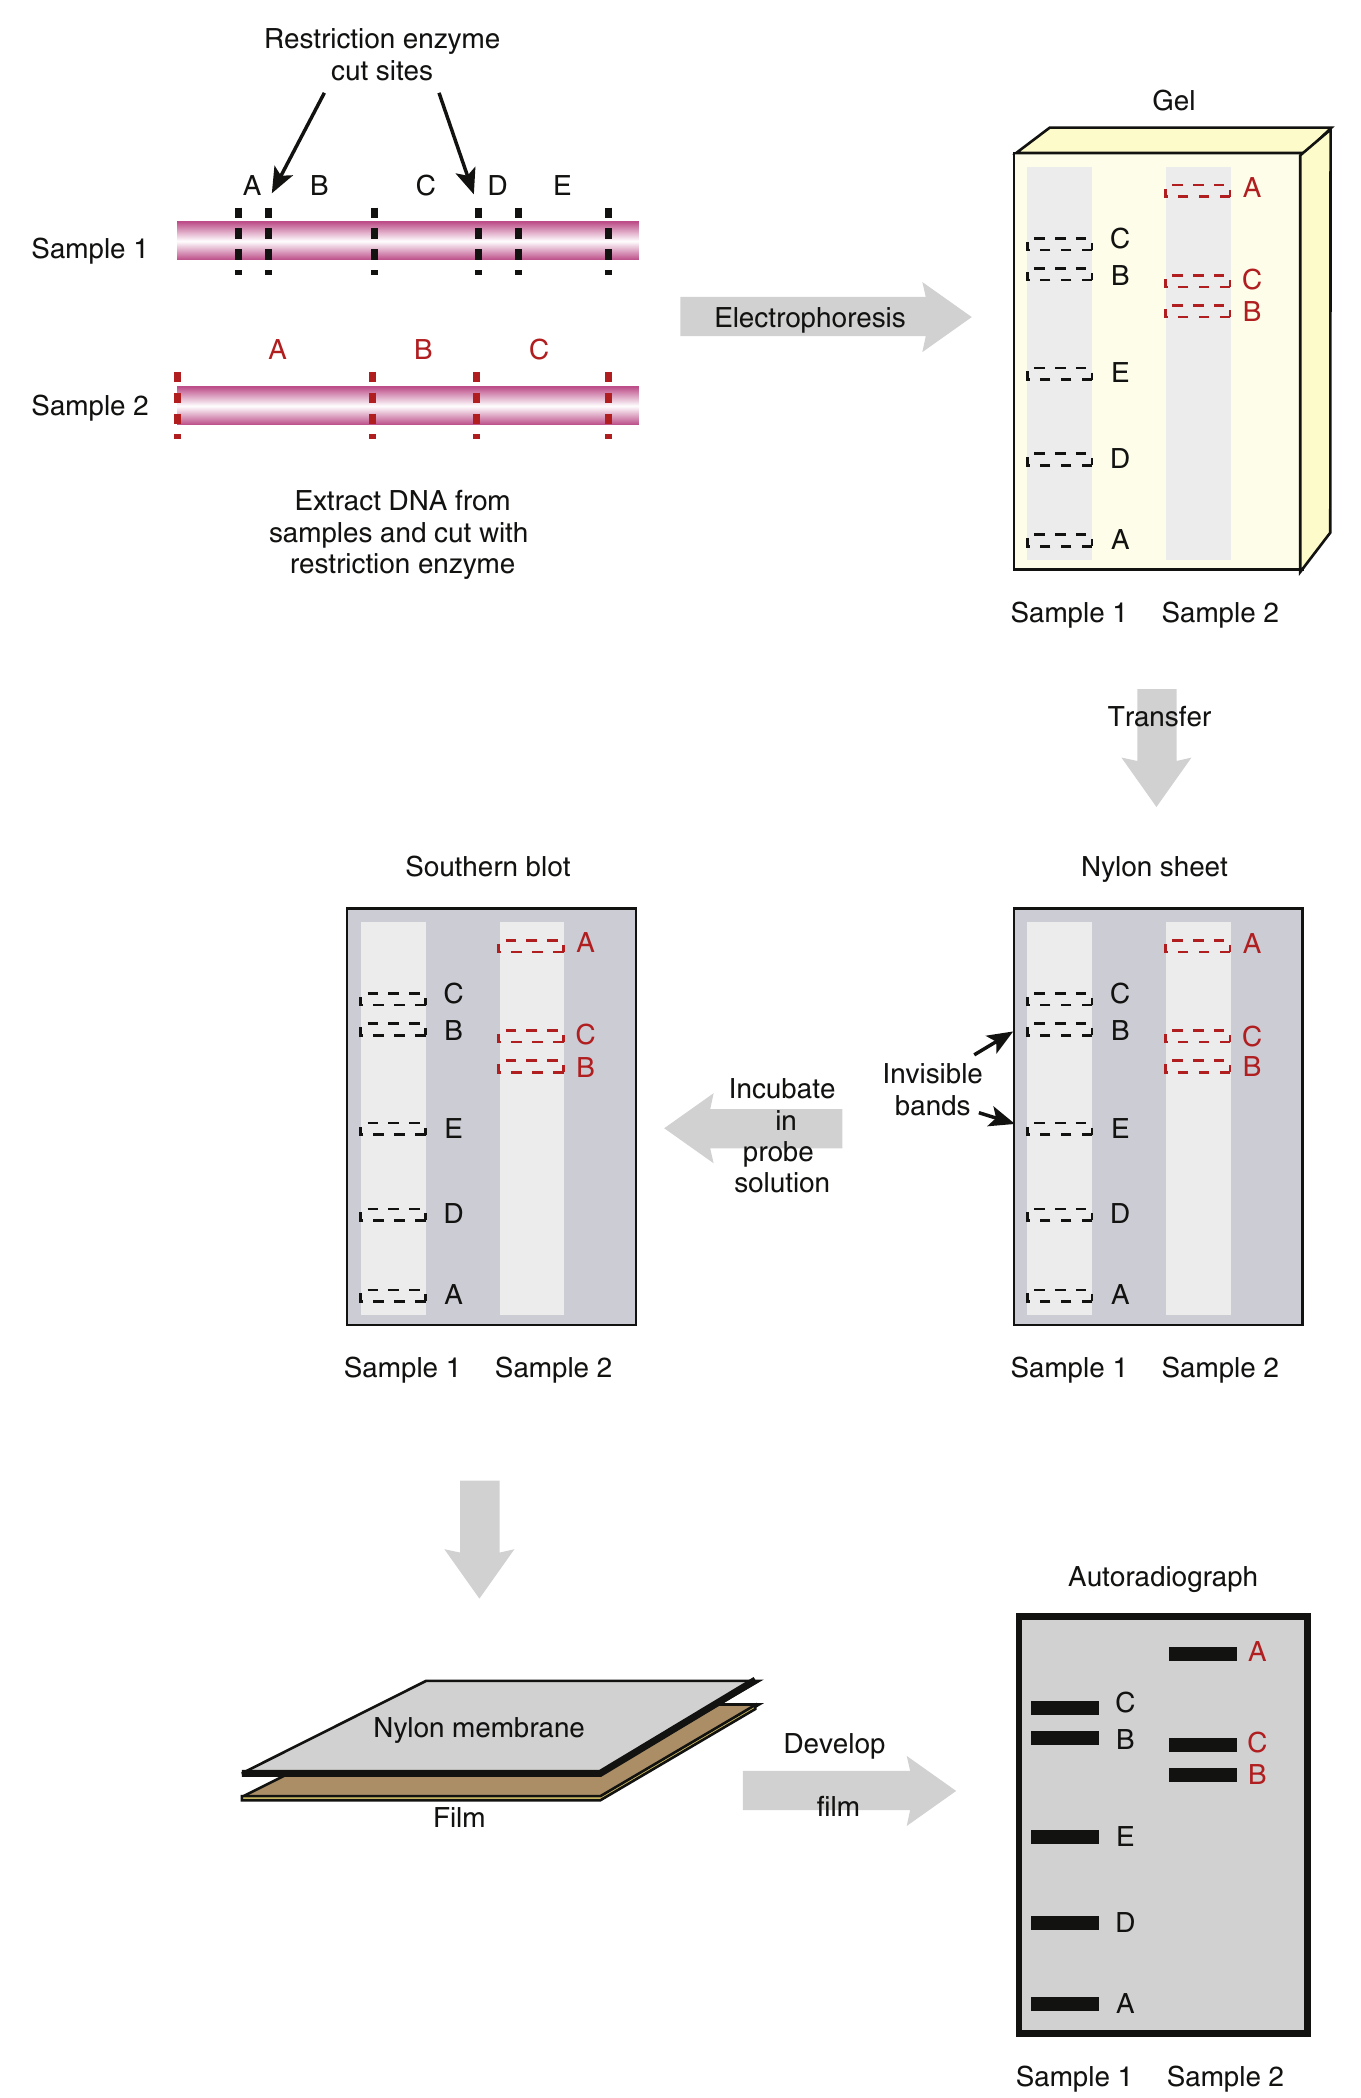
\includegraphics[width=0.32\linewidth]{../images/rflp_fingerprinting} \caption{Outline of RFLP based DNA fingerprinting}\label{fig:rflp-fingerprinting}
\end{figure}

\end{frame}

\begin{frame}{RFLP fingerprinting}
\protect\hypertarget{rflp-fingerprinting-1}{}

\begin{figure}
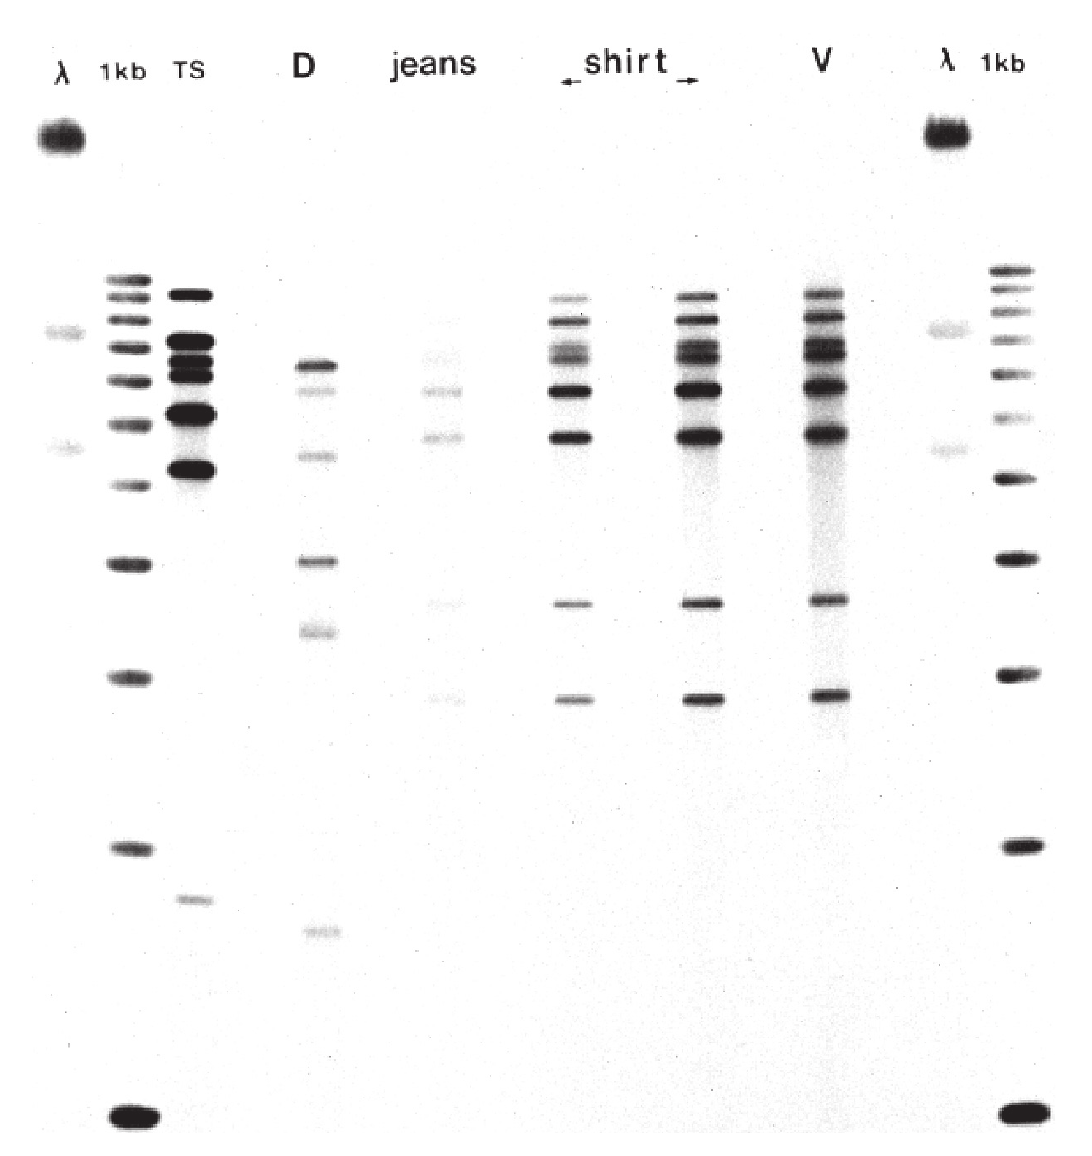
\includegraphics[width=0.4\linewidth]{../images/fingerprint_lanes} \caption{Actual DNA fingerprint showing that the pattern of DNA fragments of the victim (V) were found on the defendant's clothing (jeans/shirt). The first two and last two lanes are the standard size markers (labeled $\lambda$ and 1 kb). The lane marked TS is a positive control showing that the fingerprint technique was successful. The lane marked D is the defendant's DNA pattern.}\label{fig:fingerprint-lanes}
\end{figure}

\end{frame}

\hypertarget{bibliography}{%
\section{Bibliography}\label{bibliography}}

\end{document}
